\documentclass[xcolor=table, hyperref={pdfpagelabels=false}]{beamer}
\usepackage{lmodern}
\usepackage{amssymb}
\usepackage[style=alphabetic,
citestyle=authoryear]{biblatex}
\renewcommand*{\bibfont}{\scriptsize}
\addbibresource{bibliography.bib}

\usepackage{ulem}
\usepackage{cancel}
\usepackage{float}
\usepackage{tikz}
\usetikzlibrary{decorations.pathreplacing}
\usetikzlibrary{shapes,arrows}
\definecolor{myLightGray}{RGB}{191,191,191}
\definecolor{myGray}{RGB}{160,160,160}
\definecolor{myDarkGray}{RGB}{144,144,144}
\definecolor{myDarkRed}{RGB}{167,114,115}
\definecolor{myRed}{RGB}{255,58,70}
\definecolor{myGreen}{RGB}{0,255,71}
\usepackage{lmodern}
\usepackage{amsmath}
\usepackage{dsfont}
\usepackage{marvosym}
\usepackage{subcaption}
\usepackage{ stmaryrd }
\usepackage{refcount}


\usepackage[utf8]{inputenc}
\usetheme{Frankfurt}
\usepackage{qtree}
\usepackage{subcaption}
\newcommand\SmallCaption[1]{%
	\captionsetup{font=scriptsize}%
	\caption{#1}}

\newcommand\sqref[1]{%
	\tikz \node[rectangle, fill=structure.fg, inner sep=0pt, minimum size=3mm,
	text width=8pt,font=\scriptsize,align=center] {\color{white}\ref{#1}};
}



\title{Semantics and pragmatics of numerical approximation expressions}  
\author[a]{Adèle Mortier\\[10mm]{\small Supervisors:\\ Paul Égré $|$ Benjamin Spector}}

\date{\today} 
\begin{document}

\begin{frame}
\titlepage
\end{frame} 

\begin{frame}{Introduction: why use \textit{around}?}
\begin{block}{Numerical approximation?}
Approximation expressions: \textit{around n}, \textit{almost n}, \textit{between n and m}...\pause
\end{block}
\begin{enumerate}
	\setbeamertemplate{enumerate items}[square]
	\item \label{ite:between2832} She is between 28 and 32 y.o.
	\item \label{ite:around30} She is around 30 y.o.
	\label{end-enumerate}
\end{enumerate}
\pause
\begin{block}{\textit{Around vs between}}
	\begin{itemize}
		\item \sqref{ite:between2832} provides clear boundaries, and has a disjunctive force (\textbf{imprecision}). The speaker isn't sure about the age. \pause
		\item \sqref{ite:around30} puts focus on one number, without specifying the boundaries (\textbf{vagueness}). Either the speaker is not sure, or he knows the age but is too ``lazy'' to give the exact number. \pause
		\item hypothesis: \textit{around} gives ``something more'' about one's epistemic sate and one's priors (\cite{Egre2018pres}).
	\end{itemize}
\end{block}
\end{frame}

\iffalse
\begin{frame}{Introduction: \textit{around} and the slippery slope}
``Hong Kong Protests: around 2 Million Marchers Hit the Streets'' (\textit{Bloomberg}, June 16, 2019)
\begin{block}{What to think of this}
	\begin{itemize}
		\item Bloomberg said \textit{around}, so 1 999 999 should be fine;
		\item but since 1 999 999 is fine, 1 999 998 should be fine too
		\item ...
		\item so, it should be fine to say that 0 people  hit the streets... and the Hong Kong protest never existed!
	\end{itemize}
\end{block}
\begin{alertblock}{What to do?}
	\begin{itemize}
		\item define a sharp boundary, as in the case of \textit{between}? Weird.
		\item use probabilities to account for uncertainty about the truth or falsity of the number. \textbf{This is what we intend to do}.
	\end{itemize}
\end{alertblock}
\end{frame}
\fi
\begin{frame}
\frametitle{Table of contents}
\tableofcontents
\end{frame} 
\section{Key parameters of \textit{around}}
\begin{frame}{}
\begin{center}
	\Huge Key parameters
	\normalsize
	\begin{block}{Plan}
		\begin{itemize}
			\item ``The bigger the wider''
			\item ``The coarser the wider''
		\end{itemize}
	\end{block}
\end{center}
\end{frame}
\subsection{Order of magnitude}
\begin{frame}{Order of magnitude \small (\cite{Egre2018pres})}
\begin{minipage}{.55\textwidth}
	Introspective judgments:
	\begin{enumerate}
		\setbeamertemplate{enumerate items}[square]
		\setcounterref{enumi}{end-enumerate}
		\item He bought this sandwich for about 4\EUR $\leadsto [3.5; 4.5]$
		\item He launched the reform for a cost of about 10 bn \EUR $\leadsto [8\mbox{bn}; 12\mbox{bn}]$
		\label{end-enumerate}
	\end{enumerate}\pause
	\hspace*{-12mm}
	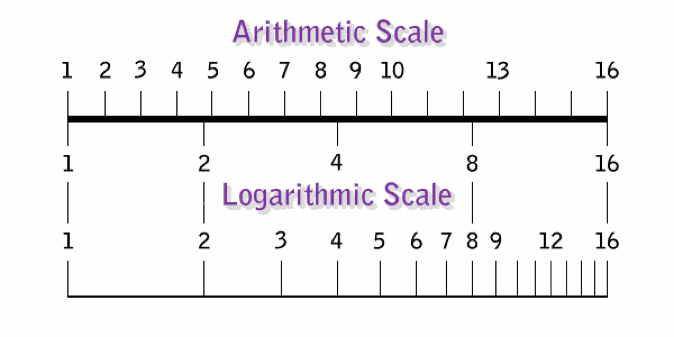
\includegraphics[width=1.2\textwidth]{./images/log_scale.png}
\end{minipage}
\begin{minipage}{.4\textwidth}
	\begin{block}{Intuition (\cite{Dehaene2003})}
		\begin{itemize}
			\item on a \textbf{log scale}, perceived spacing between consecutive numbers is ``distorted'';
			\item bigger numbers means smaller spacing;
			\item so, a fixed-size interval contains more big numbers than small numbers
		\end{itemize}
	\end{block}
\end{minipage}
\end{frame}
\subsection{Granularity}
\begin{frame}{Granularity \small (\cite{Cummins2012,Zhang2012})}
\begin{minipage}{\textwidth}
	Introspective judgments:
\begin{enumerate}
	\setbeamertemplate{enumerate items}[square]
	\setcounterref{enumi}{end-enumerate}
	\item \label{ite:100_marbles}She has around 20 marbles in her bag $\leadsto [16; 24]$
	\item \label{ite:105_marbles} She has around 15 marbles in her bag $\leadsto [11; 19]$
	\item \label{ite:101_marbles} ??She has around 17 marbles in her bag $\leadsto \lbrace 17 \rbrace??$
	\item \label{ite:101_km} She drove around 17 kilometers $\leadsto [16.1; 17.9]$
\end{enumerate}
\end{minipage}
\begin{minipage}{.45\textwidth}
	\begin{block}{Remarks}
	\begin{itemize}
		\item \sqref{ite:100_marbles}, \sqref{ite:105_marbles} and \sqref{ite:101_marbles} are very close on the log scale and yet induce different intervals;
		\item \sqref{ite:101_marbles} and \sqref{ite:101_km} feature the same number (same granularity), but \sqref{ite:101_marbles} seems infelicitous.
	\end{itemize}
\end{block}
\end{minipage}\qquad
\begin{minipage}{.45\textwidth}
	\begin{alertblock}{Two principles}
	\begin{itemize}
		\item \textbf{granularity constraint}: coarser granularity, bigger interval;
		\item \textbf{granularity violation}: when the granularity of the number is less than or equal to the minimum granularity of the scale.
	\end{itemize}
\end{alertblock}
\end{minipage}
\end{frame}
\section{Two Bayesian models}
\begin{frame}{}
\begin{center}
	\Huge Two Bayesian models
	\normalsize
	\begin{block}{Plan}
		\begin{itemize}
			\item a model inspired by the Rational Speech Acts framework accounting for granularity effect;
			\item a model based on probabilistic intervals allowing for speaker uncertainty.
		\end{itemize}
	\end{block}
\end{center}

\end{frame}
\subsection{RSA model}
\begin{frame}{A Rational Speech Acts (RSA) model}
\begin{block}{Principle  \small (\cite{Lassiter2013,Bergen2016})}
	\begin{itemize}
		\item one set of \textbf{utterances} (each with a cost and possible meanings), one set of \textbf{observations} (numbers), one set of interval \textbf{thresholds} (numbers); \pause
		\item mutually recursive Bayesian updates (``I know that you know that I know...''); \pause
		\item optimality = tradeoff between \textbf{cost} and \textbf{informativity}.
	\end{itemize}
\end{block}
\begin{figure}
	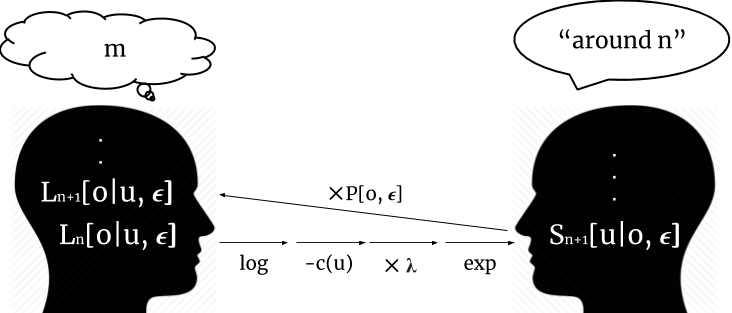
\includegraphics[width=.75\textwidth]{./images/rsa.png}
\end{figure}
\end{frame}


\begin{frame}{RSA and granularity}
\begin{minipage}{.4\textwidth}
	\begin{figure}
		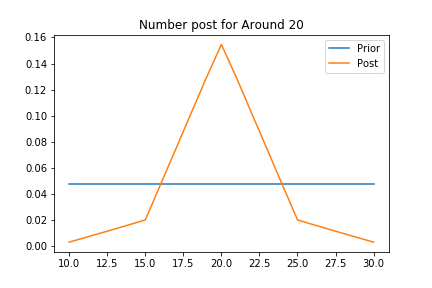
\includegraphics[width=.8\textwidth]{./images/number_post_around_20.png}
		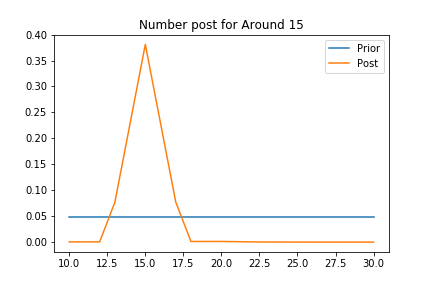
\includegraphics[width=.8\textwidth]{./images/number_post_around_15.png}
		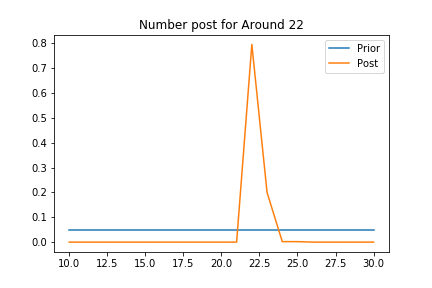
\includegraphics[width=.8\textwidth]{./images/number_post_around_22.png}
	\end{figure}
\end{minipage}
\begin{minipage}{.55\textwidth}
	 \begin{block}{The trick}
 	\begin{itemize}
 		\item granularity encoded in the \textbf{cost function}! \pause
 		\item c/i tradeoff ensures that the probability drops at the level of next coarser number (more optimal, and yet not used).
 	\end{itemize}
 \end{block}
\pause
\begin{alertblock}{Caveats}
	\begin{itemize}
		\item does not come for free... ``good'' granularity function? \pause
		\item RSA assumes that the speaker knows the exact number... not very realistic!
	\end{itemize}
\end{alertblock}
\end{minipage}

\end{frame}
\subsection{Probabilistic intervals}
\begin{frame}{Probabilistic intervals \small (\cite{Egre2018pres})}
\begin{block}{Principle: 2 levels of uncertainty}
	\begin{itemize}
		\item when the speaker utters ``around n'', he thinks of a certain interval among a \textbf{set of possible intervals} (\textit{e.g.} intervals centered around n); \pause
		\item according to the listener, \textbf{each possible interval has a certain probability} (\textit{e.g.} relatively narrow intervals might be more probable); \pause
		\item and within a fixed interval, the \textbf{``real'' number} is guessed according to a certain prior (\textit{e.g.} central numbers might be more probable)
		\item use Bayes rule!
	\end{itemize}
\end{block}
\begin{figure}
	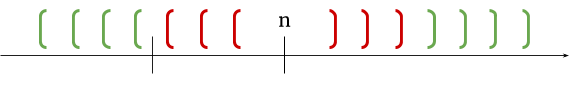
\includegraphics[width=\textwidth]{./images/intervals.png}
\end{figure}
\end{frame}
\begin{frame}{A simulation with uniform priors}\vspace{-3mm}
\begin{figure}
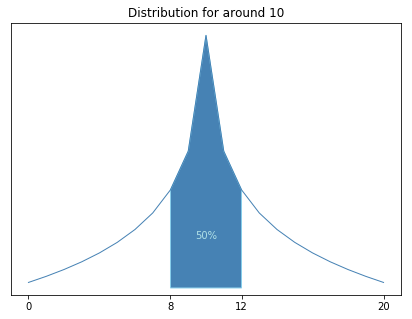
\includegraphics[width=.4\textwidth]{./images/around_10_prob_simple.png}
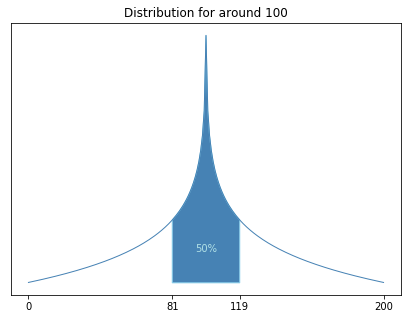
\includegraphics[width=.4\textwidth]{./images/around_100_prob_simple.png}
\caption{Curves generated using uniform distributions on intervals and numbers}
\end{figure}
\vspace{-8mm}
\begin{block}{Properties}
\begin{itemize}
	\item Symmetrical, scales with magnitude, not granularity \pause
	\item \textbf{Increases the probability discrepancy between central and peripheral numbers} (posterior is more peaked than prior)... does \textit{not} depend on priors. 
\end{itemize}
\end{block}
\end{frame}

\section{Experiments}
\begin{frame}{}
\begin{center}
	\Huge Experiments
\end{center}
\end{frame}
\begin{frame}{Goals}
\begin{block}{What}
	\begin{itemize}
		\item ``(Around$|$between$|$almost...) $n$ people came to the party''; \pause
		\item elicitation of \textbf{intervals of possible values} \small(\cite{Channell1994}...) \normalsize; \pause
		\item elicitation of \textbf{probability distributions} ont these intervals. \pause
	\end{itemize}
\end{block}\vspace{-2mm}
\begin{figure}
	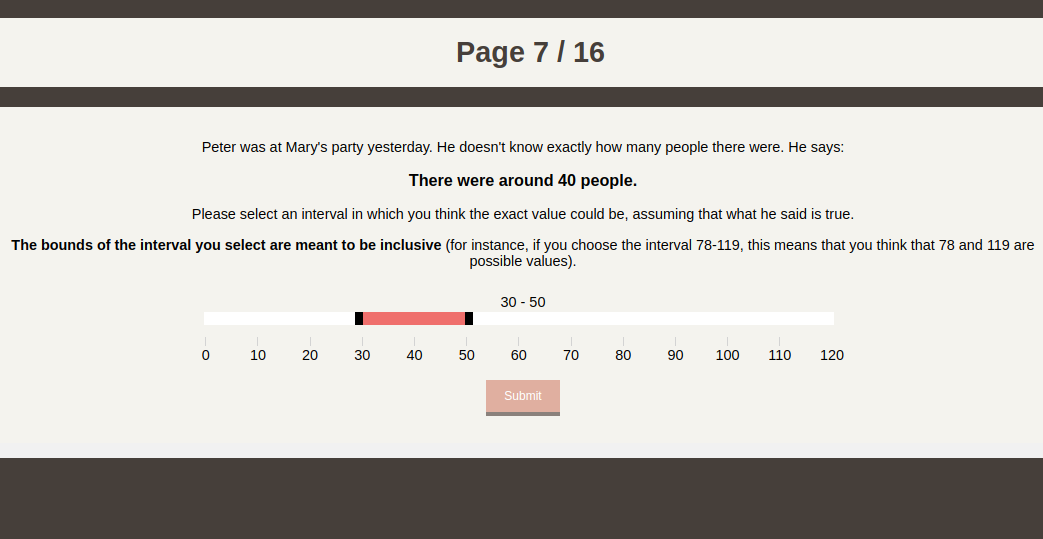
\includegraphics[width=.45\textwidth]{./images/screen_int.png} \quad
	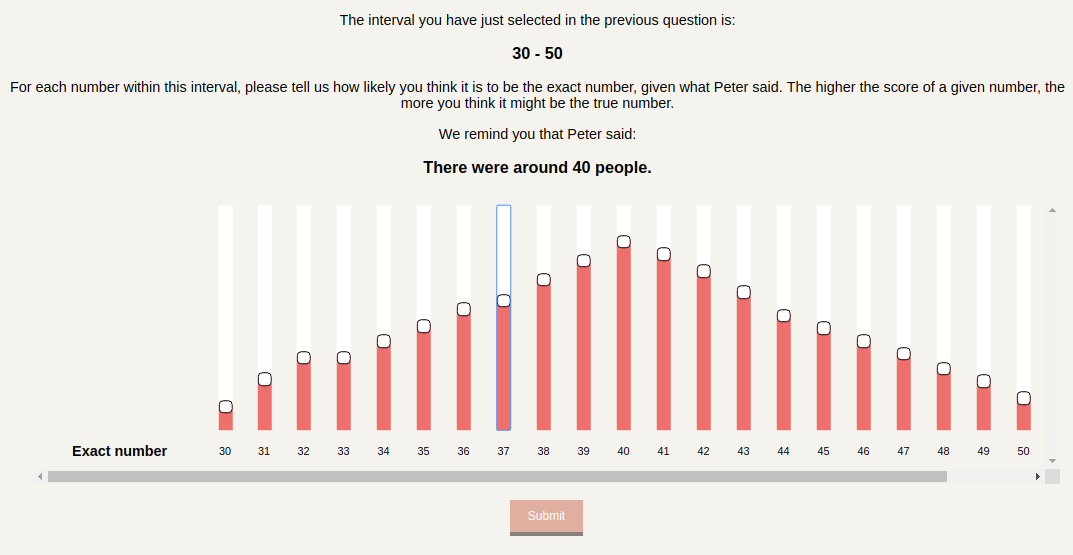
\includegraphics[width=.45\textwidth]{./images/screen_hist.png}
\end{figure}\vspace{-5mm} \pause
\begin{block}{Why}
	\begin{itemize}
		\item to check the basic features of \textit{around}; \pause
		\item to compare \textit{around} and \textit{between} and \textbf{validate the model}.
	\end{itemize}
\end{block}
\end{frame}

\begin{frame}{Hypotheses and issues}
\begin{block}{Hypotheses}
	\begin{itemize}
		\item with \textit{\textbf{between}}, the interval is already known, the listener simply uses the \textbf{prior} on it; \pause
		\item with \textit{\textbf{around}}, the interval is not known, the listener conditionalizes over multiple nested intervals, which mechanically increases the peakedness of the distribution (\textbf{post}); \pause
		\item therefore, \textbf{the \textit{around}-distribution must be more peaked than the \textit{between}-distribution}!
	\end{itemize}
\end{block}\pause
\begin{alertblock}{Issues}
	\begin{itemize}
		\item \textbf{target items}: which expressions should we compare? \pause
		\item \textbf{prediction}: what should we measure and test? \pause
		\item \textbf{design}: who sees what and when?
	\end{itemize}
\end{alertblock}
\end{frame}
\subsection{Items}
\begin{frame}{Target items}
\begin{block}{\textit{around n vs between x and y}}
	\begin{itemize}
		\item we should better compare distributions defined on the \textbf{same set of possible numbers}...\pause
		\item but the participants are free to choose the domain of their distributions! \pause
		\item we can somewhat ``force'' domain equality by \textbf{dynamically determining the target \textit{between} item}; \pause
		\item but then, we cannot control for \textbf{order effects}...
	\end{itemize}
\end{block}
\begin{table}
	\centering
	\begin{tabular}{ccc}
	Question && Answer \\
	``Around 40?'' &$\rightarrow$ & $[$\textbf{32}; \textbf{48}$]$ \\
	Fillers &$\rightarrow$ & ... \\
	``Between \textbf{32} and \textbf{48}?'' &$\rightarrow$& $[32;48]$
\end{tabular}
\end{table}
\end{frame}
\subsection{Metric}
\begin{frame}{Metric}
\begin{block}{Model prediction}
	\begin{itemize}
		\item the model predicted an increase of peakedness after hearing \textit{around}, no matter the prior distribution; \pause
		\item this translates into: \textbf{$\frac{Post(k)}{Post(k')} \geq \frac{Prior(k)}{Prior(k')}$} when $k$ is more central than $k'$; \pause
		\item the \textit{Post} distribution is induced by \textit{around}; while the \textit{Prior} distribution is induced by \textit{between}.
	\end{itemize}
\end{block}\pause
\begin{alertblock}{Caveats}
	\begin{itemize}
		\item best is to compare very distant numbers, but we should also avoid division by 0 and the use of salient numbers! \pause
		\item we should compare probabilities of numbers that are defined in both the \textit{between} and \textit{around} distributions at stake; \pause
		\item we should average multiple ratios to increase robustness.
	\end{itemize}
\end{alertblock}
\end{frame}
\subsection{Design}
\begin{frame}{Design}
\begin{block}{Matched \textit{vs} unmatched}
	\begin{itemize}
		\item \textbf{matched-pairs}: comparing distributions defined on very similar domains becomes easier;
		\item \textbf{unmatched groups}: using averaged distributions may play in favor of our hypothesis for the wrong reasons
		\item indeed, when uniform distributions coming from different participants are ``piled up'', it creates a peaked distribution! 
	\end{itemize}
\end{block}
\begin{figure}
	\centering
	\begin{subfigure}[t]{.45\textwidth}
		\centering
		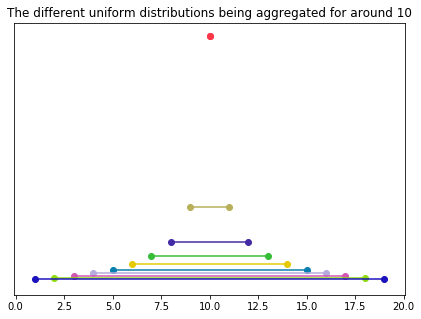
\includegraphics[width=.6\textwidth]{./images/around_10_prob_simple_aggregate.png}
		\SmallCaption{What happens in the model}
	\end{subfigure}
	\begin{subfigure}[t]{.45\textwidth}
		\centering
		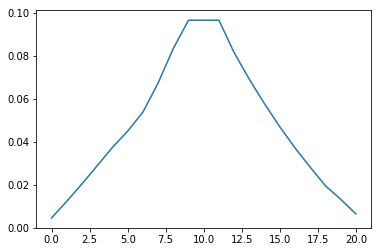
\includegraphics[width=.6\textwidth]{./images/sim_aggregated_mildly_peaked.png}
		\SmallCaption{What could happen with the data}
	\end{subfigure}
	\SmallCaption{An unmatched design would emulate what happens at the individual level in the model using inter-individual data: big confusion!}
\end{figure}
\end{frame}
\begin{frame}{Summary}
\begin{block}{Pilots}
	\begin{itemize}
		\item first pilot (n=20): assess interval width and inter-subject variability, select target numbers; \pause
		\item three other pilots (n=15 each): collect subjective probability distributions with varying items, orders, input modes. See what gives the best performances.
	\end{itemize}
\end{block} \pause
\begin{block}{Main experiment}
	\begin{itemize}
		\item ask 200 participants about \textit{around}, \textit{between} and \textit{almost}; \pause
		\item three possible numbers for the target trial: around 40, 50 or 60; \pause
		\item target items in fixed positions, randomized fillers; \pause
		\item target \textit{between} item generated dynamically after \textit{around}.
	\end{itemize}
\end{block}
\end{frame}
\section{Results}
\begin{frame}{}
\begin{center}
	\Huge Results
\end{center}
\end{frame}
\subsection{Pre-registered}
\begin{frame}{First pilot}
\begin{figure}
	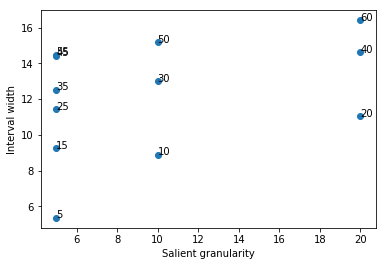
\includegraphics[width=.45\textwidth]{./images/pilote_1_av_width_by_g.png}
	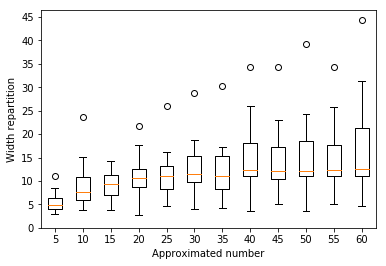
\includegraphics[width=.45\textwidth]{./images/pilote_1_width_repartition.png}
\end{figure}
\begin{block}{Observations}
	\begin{itemize}
		\item effect of \textbf{granularity}: close numbers with different intrinsinc salient granularities give rise to different intervals (\textbf{coarser = wider});
		\item effect of \textbf{order of magnitude}: distant numbers with same granularity give rise to different intervals (\textbf{bigger = wider}); bigger numbers also give rise to more variable intervals.
	\end{itemize}
\end{block}
\end{frame}
\begin{frame}{Main experiment}
\begin{minipage}{.4\textwidth}
	\begin{figure}
		\centering
		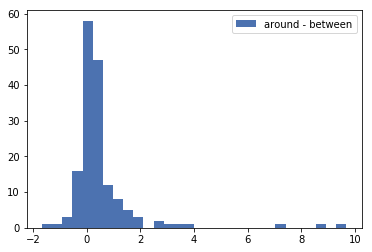
\includegraphics[width=\textwidth]{./images/main_exp_diff_dist.png}
		\SmallCaption{Repartition of the paired differences between the scores for \textit{around} and the scores for \textit{between}}
\end{figure}\pause
\end{minipage}\quad
\begin{minipage}{.55\textwidth}
	\begin{block}{Hypothesis testing}
	\begin{itemize}
		\item Wilcoxon signed-rank test for matched pairs
		\item Significant difference between the scores for \textit{around} and the scores for \textit{between} (n=162, p=$8.504 \times 10^{-13}$, effect size=0.56)
	\end{itemize}
\end{block}\pause
\end{minipage}
\begin{alertblock}{Interpretation}
	\begin{itemize}
		\item however, we cannot be sure that the effect is really due to a subjective difference between the two approximators...\pause
		\item indeed, order effects were not controlled... \pause
		\item and the variability of the number could have interfered.
	\end{itemize}
\end{alertblock}
\end{frame}
\subsection{Exploratory analyses}
\begin{frame}{Exploratory analysis -- Number effect (thanks to Steven Verheyen)}
	\begin{block}{Number-by-number analysis}
		\begin{itemize}
			\item participants were assigned randomly to 3 possible target numbers: 40, 50, 60;
			\item but the distribution of scores may vary with the number, \textit{i.e.} one number ``weighs more'' in the test;
			\item we did three separate analyses to check that.
		\end{itemize}
	\end{block}
\begin{minipage}{.52\textwidth}
	\begin{figure}
	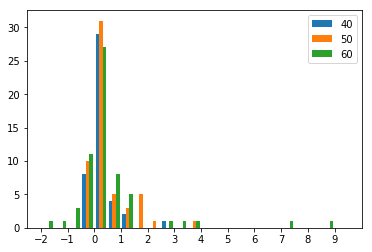
\includegraphics[width=\textwidth]{./images/dist_scores_by_number.png}
\end{figure}
\end{minipage}
\begin{minipage}{.43\textwidth}
	\setlength\tabcolsep{3pt}  % default value: 6pt
	\tiny
	\begin{table}
	\begin{tabular}{c|ccc}
		Number & 40 & 50 & 60 \\ \hline
		Sample & 44 & 57 & 61 \\
		Median & 0.13 & 0.27 & 0.30 \\
		Std & 0.50 & 1.42 & 1.60 \\
		p-value & $4.32 \times 10^{-4}$ & $2.35 \times 10^{-6}$ & $3.15 \times 10^{-4}$
	\end{tabular}
\end{table}
\end{minipage}
\end{frame}
\begin{frame}{Exploratory analysis -- Order effects}
\begin{block}{Assessing order effects}
	\begin{itemize}
	\item ``quick and dirty'' analysis to verify whether order effects may explain a significant part of what has been observed;
	\item comparison of filler items (\textit{around} and \textit{between}) depending on their position in the survey (randomized over participants);
	\item participants become more and more uniform with time!
\end{itemize}
\end{block}
\begin{figure}
	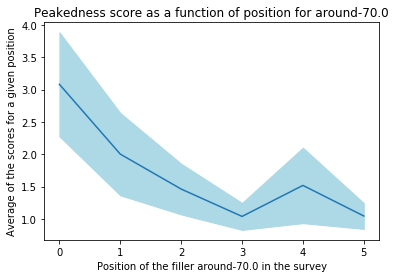
\includegraphics[height=100px]{./images/evol_peakedness_around_70.png}
	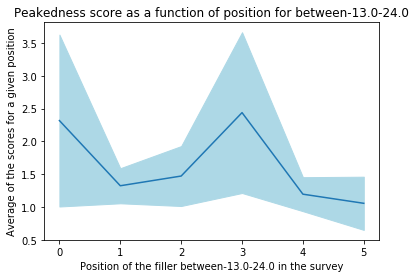
\includegraphics[height=100px]{./images/evol_peakedness_between_13_24.png}
\end{figure}
\end{frame}

\section{Conclusion}
\begin{frame}{Conclusion}
	\begin{alertblock}{A mixed picture}
		\begin{itemize}
			\item our results lack robustness; \pause
			\item our custom score is difficult to interpret, because its properties are largely unknown. \pause
		\end{itemize}
	\end{alertblock}

	\begin{exampleblock}{What's next?}
		\begin{itemize}
			\item starting from the PI model, develop a more refined model dealing with \textit{both} speaker uncertainty and granularity; \pause
			\item better control for order effects, which leads to go back to a static design and use a more  appropriate model (mixed model).
		\end{itemize}
	\end{exampleblock}

\end{frame}
\begin{frame}[allowframebreaks]
\frametitle{Selected references}
\nocite{*}

\printbibliography
\end{frame}

\section{Appendices}
\begin{frame}{Additional data (many thanks to Steven Verheyen)}
About intervals and social constraints:
\begin{enumerate}
	\setbeamertemplate{enumerate items}[square]
	\item -- I ate around 10 cookies... --Liar, you ate 12 of them!!
	\item -- I ate around 10 cookies... --*Liar, you ate 8 of them!!
	\item -- I helped around 10 children --*Liar, you helped 12 of them!!
	\item -- I helped around 10 children --Liar, you helped 8 of them!!
	\label{end-enumerate}
\end{enumerate}
\begin{block}{Role of valence}
	\begin{itemize}
		\item negative valence: \textit{around} closer to an upper bound (honesty)
		\item positive valence: \textit{around} closer to a lower bound (humility)
	\end{itemize}
\end{block}

\end{frame}

\begin{frame}{Additional data (inspired from \cite{Zhang2012})}
\begin{minipage}{.55\textwidth}
	\begin{enumerate}
	\setbeamertemplate{enumerate items}[square]
	\setcounterref{enumi}{end-enumerate}
	\item I ran around 1.5 km
	\item I ran around 15 hundred meters
	\item I ran around 15 hm
	\item I ran around 1500 m
\end{enumerate}
\begin{figure}
	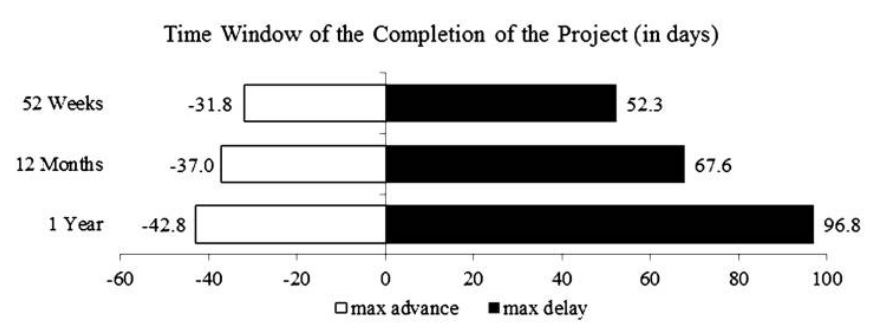
\includegraphics[width=\textwidth]{./images/zhang_data.png}
	\caption{weeks \textit{vs} months \textit{vs} years, \cite{Zhang2012}}
\end{figure}
\end{minipage}
\quad
\begin{minipage}{.4\textwidth}
	\begin{block}{Unit conveys granularity}
	\begin{itemize}
		\item coarser unit = coarser scale = less precise = less reliable;
		\item effect disappears when Gricean cooperation no longer holds;
		\item if unit is too precise, sometimes reverse effect (``too good to be true!'').
	\end{itemize}
\end{block}
\end{minipage}
\end{frame}

\begin{frame}{Proof of $W \propto n$ on log scale}
Suppose we want a interval with a fixed size $W$ around $n$, \textit{on a log scale}. For the size $W$ to remain fixed, what should be the value of the semi-width $\epsilon$, depending on $n$, on a liner scale?
\begin{eqnarray*}
	Size([n-\epsilon; n+\epsilon]) = W &\iff& \log\left(\frac{n+\epsilon}{n-\epsilon}\right) \propto W \\
	&\iff& \frac{n+\epsilon}{n-\epsilon} \propto \exp(W)\\
	&\iff& n+ \epsilon \propto \exp(W)(n-\epsilon)\\
	&\iff& \epsilon(1+\exp(W)) \propto n(\exp(W)-1)\\
	&\iff& \epsilon \propto \frac{n(\exp(W)-1)}{1+\exp(W)}\\
	&\iff& \epsilon \propto n
\end{eqnarray*}
\end{frame}

\begin{frame}{Granularity effects on quantified numerals \small (\cite{Cummins2012})}
\begin{minipage}{.4\textwidth}
	\begin{block}{Study}
	\begin{itemize}
		\item tested \textit{more than n} and \textit{at least n};
		\item pointwise estimate or intervals;
		\item with coarser granularities, average distance to $n$ becomes larger;
		\item effect disappears when number is primed.
	\end{itemize}
\end{block}
\end{minipage}\quad
\begin{minipage}{.55\textwidth}
	\begin{figure}
	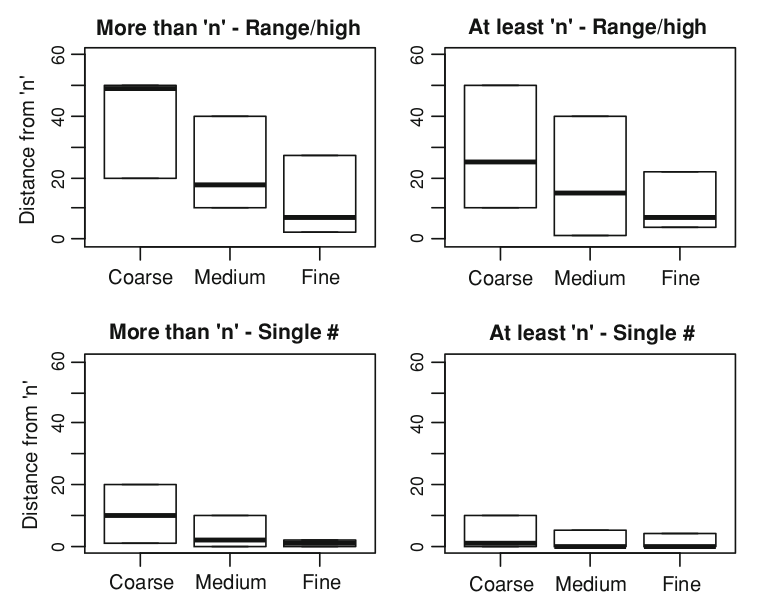
\includegraphics[width=\textwidth]{./images/cummins_data.png}
\end{figure}
\end{minipage}

\end{frame}

\begin{frame}{Granularity as exhaustification}
\begin{block}{Why granularity \textit{implicatures}?}
	\begin{itemize}
		\item granularity conveys a salient scale, potentially different from unit-induced scale: 2-by-2, 5-by-5, 10-by-10 etc.
		\item a granularity implicature is an exhaustification process pretty much alike ``\textit{exaclty}''-implicatures with bare numerals...
		\item ... but on the salient scale! (plus convexity assumption)
	\end{itemize}
\end{block}

\begin{figure}
		\begin{tikzpicture}[%
	every node/.style={
		font=\scriptsize,
		% Better alignment, see https://tex.stackexchange.com/questions/315075
		text height=1ex,
		text depth=.25ex,
	},
	]
	% draw horizontal line   
	\draw[-] (0,0) -- (10,0);
	
	% draw vertical lines
	\foreach \x in {0,1,...,10}{
		\draw (\x cm,3pt) -- (\x cm,0pt);
	}
	
	% place axis labels
	\node[anchor=north] at (0,0) {};
	\node[anchor=south] at (0,0) {10};
	
	\node[anchor=north] at (1,0) {};
	\node[anchor=south] at (1,0) {11};
	
	\node[anchor=north] at (2,0) {};
	\node[anchor=south] at (2,0) {12};
	
	\node[anchor=north] at (3,0) {};
	\node[anchor=south] at (3,0) {13};
	
	\node[anchor=north] at (4,0) {};
	\node[anchor=south] at (4,0) {14};
	
	\node[anchor=north] at (5,0) {};
	\node[anchor=south] at (5,0) {\textcolor{myRed}{15}};
	
	\node[anchor=north] at (6,0) {};
	\node[anchor=south] at (6,0) {16};
	
	\node[anchor=north] at (7,0) {};
	\node[anchor=south] at (7,0) {17};
	
	\node[anchor=north] at (8,0) {};
	\node[anchor=south] at (8,0) {18};
	
	\node[anchor=north] at (9,0) {};
	\node[anchor=south] at (9,0) {19};
	
	\node[anchor=north] at (10,0) {};
	\node[anchor=south] at (10,0) {20};
	\end{tikzpicture}
	\begin{tikzpicture}[%
	every node/.style={
		font=\scriptsize,
		% Better alignment, see https://tex.stackexchange.com/questions/315075
		text height=1ex,
		text depth=.25ex,
	},
	]
	% draw horizontal line   
	\draw[-] (0,0) -- (10,0);
	
	% draw vertical lines

	\draw (0 cm,3pt) -- (0 cm,0pt);
	\draw (10 cm,3pt) -- (10 cm,0pt);
	\draw (5 cm,3pt) -- (5 cm,0pt);
	
	% place axis labels
	\node[anchor=north] at (0,0) {};
	\node[anchor=south] at (0,0) {\sout{10}};
	
	
	\node[anchor=north] at (5,0) {};
	\node[anchor=south] at (5,0) {\textcolor{myRed}{15}};
	
	
	\node[anchor=north] at (10,0) {};
	\node[anchor=south] at (10,0) {\sout{20}};
	\end{tikzpicture}
	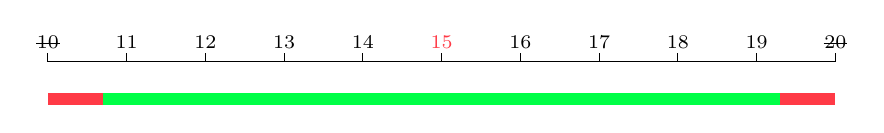
\begin{tikzpicture}[%
	every node/.style={
		font=\scriptsize,
		% Better alignment, see https://tex.stackexchange.com/questions/315075
		text height=1ex,
		text depth=.25ex,
	},
	]
	% draw horizontal line   
	\draw[-] (0,0) -- (10,0);
	
	% draw vertical lines
	\foreach \x in {0,1,...,10}{
		\draw (\x cm,3pt) -- (\x cm,0pt);
	}
	
	% place axis labels
	\node[anchor=north] at (0,0) {};
	\node[anchor=south] at (0,0) {\sout{10}};
	
	\node[anchor=north] at (1,0) {};
	\node[anchor=south] at (1,0) {11};
	
	\node[anchor=north] at (2,0) {};
	\node[anchor=south] at (2,0) {12};
	
	\node[anchor=north] at (3,0) {};
	\node[anchor=south] at (3,0) {13};
	
	\node[anchor=north] at (4,0) {};
	\node[anchor=south] at (4,0) {14};
	
	\node[anchor=north] at (5,0) {};
	\node[anchor=south] at (5,0) {\textcolor{myRed}{15}};
	
	\node[anchor=north] at (6,0) {};
	\node[anchor=south] at (6,0) {16};
	
	\node[anchor=north] at (7,0) {};
	\node[anchor=south] at (7,0) {17};
	
	\node[anchor=north] at (8,0) {};
	\node[anchor=south] at (8,0) {18};
	
	\node[anchor=north] at (9,0) {};
	\node[anchor=south] at (9,0) {19};
	
	\node[anchor=north] at (10,0) {};
	\node[anchor=south] at (10,0) {\sout{20}};
		% draw scale below
	\fill[myGreen] (0.7,-0.4) rectangle (9.3,-0.55);
	\fill[myRed] (0,-0.4) rectangle (0.7,-0.55);
	\fill[myRed] (9.3,-0.4) rectangle (10,-0.55);
	\end{tikzpicture}
	\caption{Granularity implicature for \textit{around 15}: exhaustification on a 5-by-5 scale, then back to 1-by-1 scale (scale assumed for the given unit)}
\end{figure}
\end{frame}


\begin{frame}{Probabilistic unconstrained intervals}
\begin{figure}
	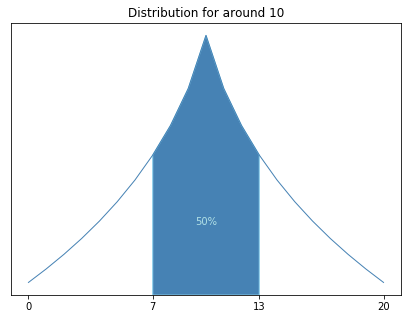
\includegraphics[width=.45\textwidth]{./images/around_10_prob_unconstrained.png}
	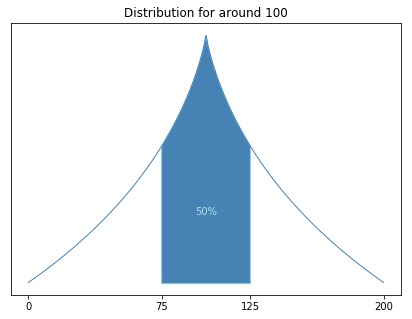
\includegraphics[width=.45\textwidth]{./images/around_100_prob_unconstrained.png}
\end{figure}

\begin{block}{Properties}
	\begin{itemize}
		\item intervals containing $n$, but not necessarily centered around $n$;
		\item scales with magnitude;
		\item less peaked.
	\end{itemize}
\end{block}
\end{frame}
\begin{frame}{RSA formulae}
\begin{equation*}
\begin{array}{rclr}
\mathds{L}_0[k|u, \epsilon] &\propto& \mathds{1}_{\lbrace k \star \epsilon \rbrace} \mathds{L}_0[k] &\mbox{[base case]} \vspace{2mm} \\ \vspace{2mm}
\mathds{S}_1[u|k, \epsilon] &\propto& \exp \left( \lambda (\log(\mathds{L}_{0}[k|u,\epsilon]) - c(u))\right) & \mbox{[inductive case]}\\ \vspace{2mm}

\mathds{L}_1[k, \epsilon|u] &\propto& \mathds{S}_N[u|k, \epsilon] \mathds{L}_0[k,\epsilon] & \mbox{[inductive case]}\\
\mathds{L}_1[k|u] &\propto& \sum_{\epsilon}\mathds{L}_1[k, \epsilon|u] \mathds{L}_0[\epsilon] & \mbox{[``Post on k'']}\\
\mathds{L}_1[\epsilon|u] &\propto& \sum_{k}\mathds{L}_1[k, \epsilon|u] \mathds{L}_0[k] & \mbox{[``Post on $\epsilon$'']}\\
\end{array}
\end{equation*}

\begin{block}{Explanations}
	\begin{itemize}
		\item first step: for fixed u (e.g. ``around x'') and $\epsilon$, just keep the observations that are in [n-$\epsilon$; n+$\epsilon$]; all the other have 0 probability.
		\item speaker step: the softmax allows to pick some non optimal possibilities with a non-zero (but very small) probability
	\end{itemize}
\end{block}
\end{frame}
\begin{frame}{RSA with quantifiers (replication)}
\begin{minipage}{.5\textwidth}
	\begin{figure}
	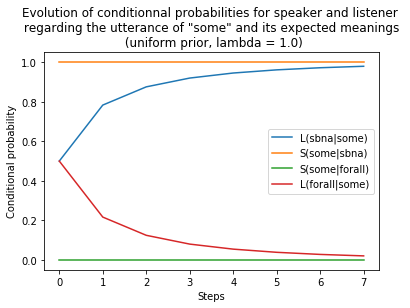
\includegraphics[width=\textwidth]{./images/quantification_lambda_1.png}
\end{figure}
\end{minipage}
\begin{minipage}{.48\textwidth}
	\begin{block}{Some \textit{vs} all}
	\begin{itemize}
		\item at the beginning, ``some'' can mean all ($\forall$) are some but not all ($\exists_{\neg \forall}$), and ``all'' definitely means $\forall$.
		\item this asymmetry causes the meaning of ``some'' to converge to $\exists_{\neg \forall}$ after a few iterations.
	\end{itemize}
\end{block}
\end{minipage}
\begin{alertblock}{\textit{Caveats}}
	\begin{itemize}
		\item Sensitive to parameter $\lambda$!
		\item $\lambda$ is the temperature, higher $\lambda$ means faster convergence but possibly to a ``wrong'' optimum.
	\end{itemize}
\end{alertblock}
\end{frame}
\begin{frame}{RSA with gradable adjectives (replication)}\vspace{-3mm}
\begin{figure}
		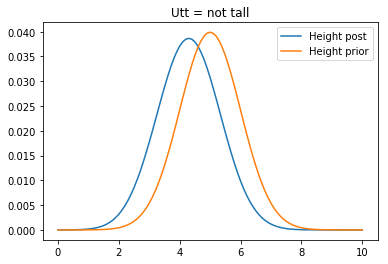
\includegraphics[width=.45\textwidth]{./images/unilateral_not_tall_height.png}
		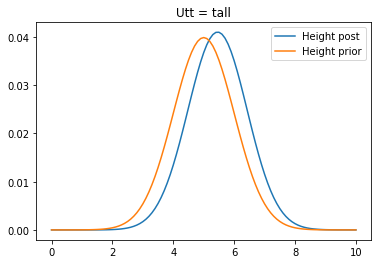
\includegraphics[width=.45\textwidth]{./images/unilateral_tall_height.png}
\end{figure}\vspace{-6mm}
\begin{block}{Properties}
	\begin{itemize}
		\item A negative utterance (``not tall''), shifts the height prior to the \textbf{left}: the listener expects the person to be \textbf{smaller};
		\item A positive utterance (``tall''), shifts the height prior to the \textbf{right}: the listener expects the person to be \textbf{taller};
		\item ``Not tall'' has a bigger effect on the prior, because it is more costly. If it has been uttered, then the person is \textit{really} small
	\end{itemize}
\end{block}
\end{frame}

\begin{frame}{RSA with competing \textit{around} and \textit{exactly}}
\begin{minipage}{.4\textwidth}
	\begin{figure}[H]
	\centering
	\begin{subfigure}[b]{.8\textwidth}
		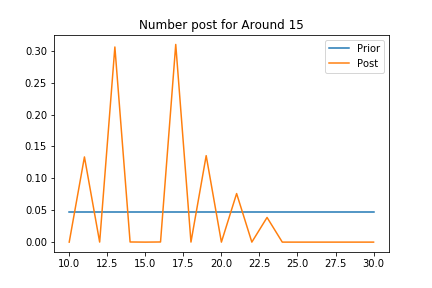
\includegraphics[width=\textwidth]{./images/number_post_around_15_exactly.png}
	\end{subfigure}
	\begin{subfigure}[b]{.8\textwidth}
		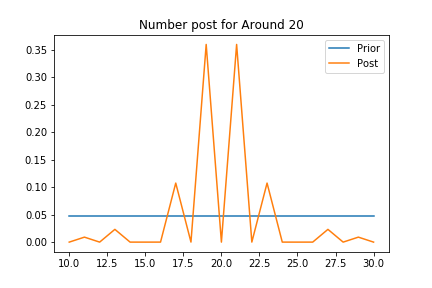
\includegraphics[width=\textwidth]{./images/number_post_around_20_exactly.png}
	\end{subfigure}
	\begin{subfigure}[b]{.8\textwidth}
		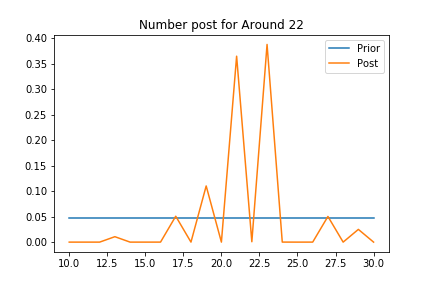
\includegraphics[width=\textwidth]{./images/number_post_around_22_exactly.png}
	\end{subfigure}
\end{figure}
\end{minipage}
\begin{minipage}{.55\textwidth}
	\begin{block}{Observations}
		\begin{itemize}
			\item ``simple'' numbers are strongly dispreferred in the interpretation of \textit{around n}, even though they are close to $n$, or even equal to $n$;
			\item indeed, saying an exact version of these numbers appears as strictly optimal, but this has not been done!
		\end{itemize}
	\end{block}
\end{minipage}
\end{frame}

\begin{frame}{RSA with competing \textit{around} and \textit{between}}
\begin{minipage}{.6\textwidth}
	\begin{figure}[H]
	\centering
	\begin{subfigure}[b]{0.45\textwidth}
		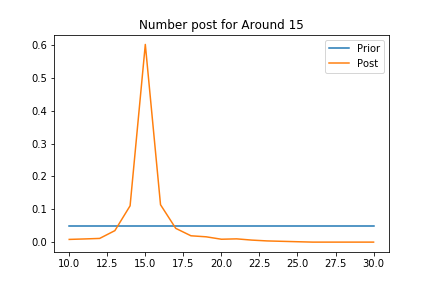
\includegraphics[width=\textwidth]{./images/number_post_around_15_between.png}
	\end{subfigure}
	\quad
	\begin{subfigure}[b]{0.45\textwidth}
		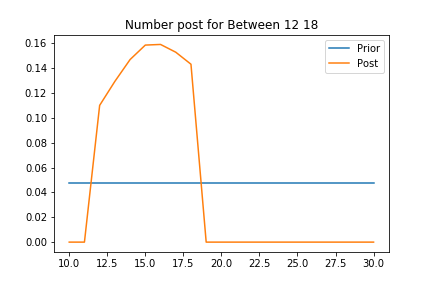
\includegraphics[width=\textwidth]{./images/number_post_between_12_18.png}
	\end{subfigure}
	
	\begin{subfigure}[b]{0.45\textwidth}
		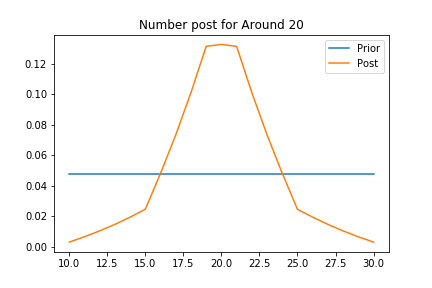
\includegraphics[width=\textwidth]{./images/number_post_around_20_between.png}
	\end{subfigure}
	\quad
	\begin{subfigure}[b]{0.45\textwidth}
		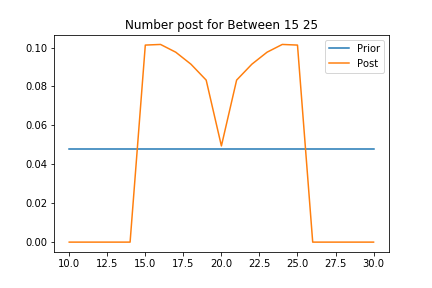
\includegraphics[width=\textwidth]{./images/number_post_between_15_25.png}
	\end{subfigure}
	
	\caption{Prior and posterior distributions for the actual number $k$, for different target numbers (15, 20) and approximators (\textit{around}, \textit{between})}
	\label{fig:rsa_approx_between}
\end{figure}
\end{minipage}
\begin{minipage}{.35\textwidth}
	\begin{block}{Observations}
		\begin{itemize}
			\item \textit{around} is very peaked as in other simulations;
			\item \textit{between} is ``anti-peaked'': if the bounds are as they are, their probability \textit{must} be high enough (otherwise, narrower bounds would have been more optimal).
		\end{itemize}
	\end{block}
\end{minipage}
\end{frame}

\begin{frame}{Arguments for a robust score (not a just one ratio)}
\begin{figure}[H]
	\centering
	\begin{subfigure}[t]{.4\textwidth}
		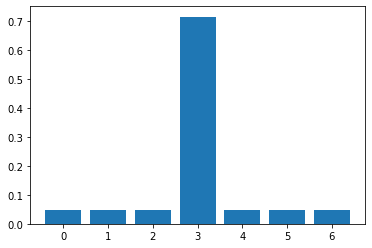
\includegraphics[width=\textwidth]{./images/true_positive.png}
		\caption{True positive, s = 15.0}
	\end{subfigure}
	\begin{subfigure}[t]{.4\textwidth}
		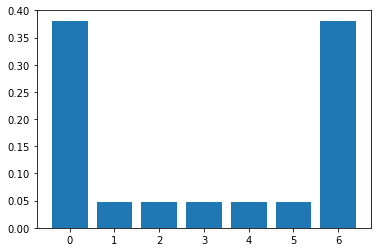
\includegraphics[width=\textwidth]{./images/true_negative.png}
		\caption{True negative, s = 0.125}
	\end{subfigure}
\end{figure}
\begin{figure}[H]\ContinuedFloat
	\centering
	\begin{subfigure}[t]{.4\textwidth}
		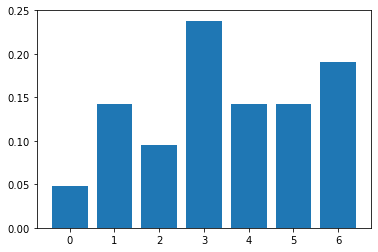
\includegraphics[width=\textwidth]{./images/false_positive.png}
		\caption{False positive, s = 5.0}
		\label{fig:false_positive}
	\end{subfigure}
	\begin{subfigure}[t]{.4\textwidth}
		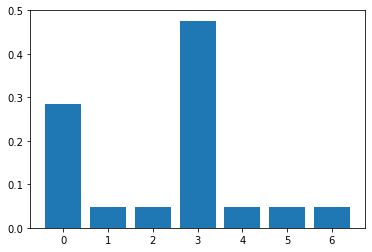
\includegraphics[width=\textwidth]{./images/false_negative.png}
		\caption{False negative, s = 1.67}
		\label{fig:false_negative}
	\end{subfigure}
	\caption{Some paradigmatic and pathological distributions w.r.t. the simple ratio score}
	\label{fig:pathological}
\end{figure}
\end{frame}

\begin{frame}{PI formula}
\begin{block}{Bayesian reasoning}
	\begin{itemize}
		\item we assume that the speaker chooses an interval in the set of all-positive intervals centered around $n$;
		\item for all $i \in [0; n]$, we call $\mathcal{A}^n_i$ the event ``speaker chooses interval $[n-i; n+i]$'';
		\item this constitutes a partition of the possible events;
		\item if we consider event $\mathcal{A}^n_i$, the probability that the speaker chooses number $k$ given $\mathcal{A}^n_i$ is $\mathcal{P}[k|\mathcal{A}^n_i]$.
		\item note that if $k < n-i$ or $k > n+i$, \textit{i.e.} $i < |n-k|$, $\mathcal{P}[k|\mathcal{A}^n_i] = 0$
	\end{itemize}
\end{block}
\tiny
\begin{equation*}
\mbox{\begin{normalsize}
	Bayes: 
	\end{normalsize}} \mathds{P}[k] = \sum_{i = 0}^n \mathcal{P}[k|\mathcal{A}^n_i] \mathds{P}[\mathcal{A}^n_i] = \bcancel{\sum_{i = 0}^{|n-k|-1} \mathcal{P}[k|\mathcal{A}^n_i] \mathds{P}[\mathcal{A}^n_i]}+\sum_{i = |n-k|}^n \mathcal{P}[k|\mathcal{A}^n_i] \mathds{P}[\mathcal{A}^n_i]
\end{equation*}
\end{frame}

\begin{frame}{Ratio inequality}
\normalsize
We assume that $|n-k| < |n-k'|$, \textit{i.e.} $k$ closer to $n$ than $k'$.
\tiny
\begin{eqnarray*}
	\frac{\mathds{P}[k|\mbox{'around n'}]}{\mathds{P}[k'|\mbox{'around n'}]} &=& \frac{\sum_{i = |n-k|}^n \mathds{P}[k|\mathcal{A}^n_i]\mathds{P}[\mathcal{A}^n_i]}{\sum_{i = |n-k'|}^n \mathds{P}[k'|\mathcal{A}^n_i]\mathds{P}[\mathcal{A}^n_i]}\\
	&=& \frac{\sum_{i = |n-k|}^{|n-k'|-1} \mathds{P}[k|\mathcal{A}^n_i]\mathds{P}[\mathcal{A}^n_i] +\sum_{i = |n-k'|}^n \mathds{P}[k|\mathcal{A}^n_i]\mathds{P}[\mathcal{A}^n_i]}{\sum_{i = |n-k'|}^n \mathds{P}[k'|\mathcal{A}^n_i]\mathds{P}[\mathcal{A}^n_i]}\\
	&\geq& \frac{\sum_{i = |n-k'|}^n \mathds{P}[k|\mathcal{A}^n_i]\mathds{P}[\mathcal{A}^n_i]}{\sum_{i = |n-k'|}^n \mathds{P}[k'|\mathcal{A}^n_i]\mathds{P}[\mathcal{A}^n_i]} \\
	&\geq& \frac{\mathds{P}[k|\mathcal{A}^n_n]\mathds{P}[\mathcal{A}^n_n]}{\mathds{P}[k'|\mathcal{A}^n_n]\mathds{P}[\mathcal{A}^n_n]} + \frac{\sum_{i = |n-k'|}^{n-1} \mathds{P}[k|\mathcal{A}^n_i]\mathds{P}[\mathcal{A}^n_i]}{\sum_{i = |n-k'|}^{n-1} \mathds{P}[k'|\mathcal{A}^n_i]\mathds{P}[\mathcal{A}^n_i]} \\
	&\geq& \frac{\mathds{P}[k|\mathcal{A}^n_n]\mathds{P}[\mathcal{A}^n_n]}{\mathds{P}[k'|\mathcal{A}^n_n]\mathds{P}[\mathcal{A}^n_n]} \\
	\frac{\mathds{P}[k|\mbox{'around n'}]}{\mathds{P}[k'|\mbox{'around n'}]} &\geq& \frac{\mathds{P}[k|\mathcal{A}^n_n]}{\mathds{P}[k'|\mathcal{A}^n_n]} \\
	\mbox{ratio of the posteriors} &\geq& \mbox{ratio of the priors}
\end{eqnarray*}
\end{frame}

\begin{frame}{Score formula}

$\mathds{A}$, $\mathds{B}$ are respectively the \textit{around} and the \textit{between} distributions. $E$ is the set of salient numbers: bounds of \textit{between} and target value of \textit{around}.
\footnotesize
\begin{eqnarray*}
	\forall x \in Supp(\mathds{A}\cap\mathds{B})&,& d(x) = |n-x| \\
	E &=& \lbrace n, min(Dom(\mathds{B})), max(Dom(\mathds{B})) \rbrace \\
	F &=& \lbrace (x, y) \in Supp(\mathds{A}\cap\mathds{B}) \ | \ d(x) < d(y) \wedge x, y \notin E \rbrace \\
	s(\mathds{P}) &=& \frac{1}{|F|} \sum_{(x, y) \in F}\frac{\mathds{P}(x)}{\mathds{P}(y)}
\end{eqnarray*}
\end{frame}

\begin{frame}{Benchmark of the scores (1)}
\begin{block}{Goal}
	\begin{itemize}
		\item compare different versions of our score with more standard metrics (mass ratio, kurtosis);
		\item use artificial distributions (uniform, Gaussian, Laplace with different std), more or less noisy (4 levels);
		\item compare how the different metrics sort the distributions.
	\end{itemize}
\end{block}
\begin{figure}[H]
	\centering
	\begin{subfigure}{.2\textwidth}
		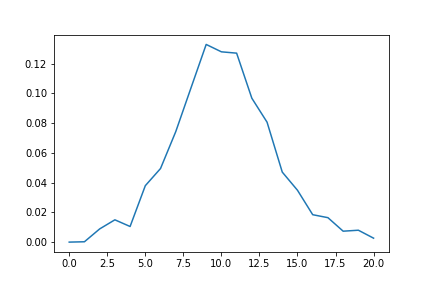
\includegraphics[width=\textwidth]{./images/5-g-3-1.png}
		\caption{Gaussian, spread=0.3, noise=0.01}
	\end{subfigure}
	\begin{subfigure}{.2\textwidth}
		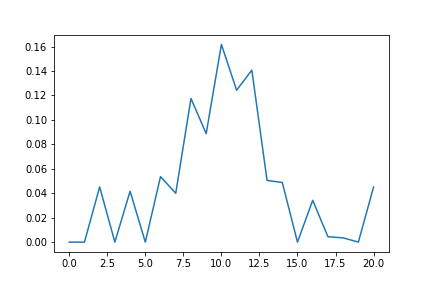
\includegraphics[width=\textwidth]{./images/11-g-3-5.png}
		\caption{Gaussian, spread=0.3, noise=0.05}
	\end{subfigure}
	\begin{subfigure}{.2\textwidth}
		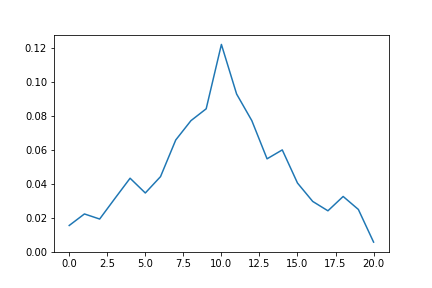
\includegraphics[width=\textwidth]{./images/13-l-5-1.png}
		\caption{Laplace, spread=0.3, noise=0.01}
	\end{subfigure}
	\begin{subfigure}{.2\textwidth}
		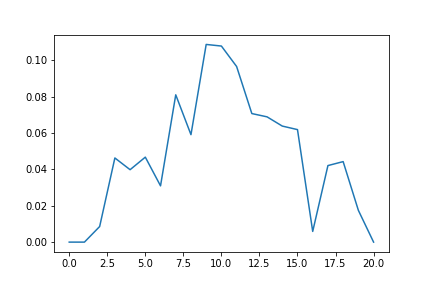
\includegraphics[width=\textwidth]{./images/6-l-5-5.png}
		\caption{Laplace, spread=0.3, noise=0.05}
	\end{subfigure}
	\caption{Example of noisy distributions generated for benchmarking the peakedness scores}
\end{figure}
\end{frame}

\begin{frame}{Benchmark of the scores (2)}
\begin{minipage}{.45\textwidth}
	\begin{table}[H]
		\centering
		\begin{tabular}{l|c}
			Score & Transpositions\\ \hline
			Simple ratio & 17 \\
			Averaged ratio & 16 \\
			Mass ratio & 15 \\
			Kurtosis & 14
		\end{tabular}
		\SmallCaption{Number of transpositions needed to change the ordering induced by a given score into the ``gold-standard'' ordering.}
		\label{tab:benchmark_scores}
	\end{table}
\end{minipage}\quad
\begin{minipage}{.5\textwidth}
	\begin{figure}[H]
		\centering
		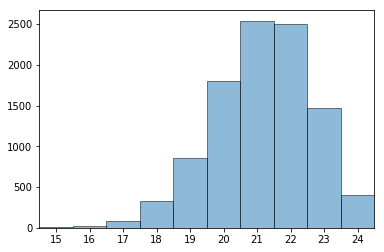
\includegraphics[width=.8\textwidth]{./images/hist_transpositions.png}
		\SmallCaption{Distribution of the number of transposition needed to transform a random permutation of size 25 into the identity permutation (10,000 trials)}
		\label{fig:random_permutation}
	\end{figure}
\end{minipage}
\vspace{-3mm}
\begin{alertblock}{Alternative}
	\begin{itemize}
		\item number of transpositions gives the same importance to ``big'' swaps and to ``small'' swaps;
		\item by using the sum of the distances between each item and its position in the ``gold standard'' ordering, we take these effects into account...
	\end{itemize}
\end{alertblock}
\end{frame}

\begin{frame}{Designs (pilots)}
\setlength\tabcolsep{1pt}  % default value: 6pt
\tiny  %%  command to change the font size
\begin{table}[H]
	\centering
	\begin{tabular}{c|c|c|c|c|c}
		Block & Numbers & Conveyed g & Critical trials & Control trials & Total\\ \hline
		Block 1 & $\lbrace$20, 40, 60$\rbrace$ & 20 & 3 & 3 & 6\\
		Block 2 & $\lbrace$20, 40, 60$\rbrace$ & 20 & 6 & 3 & 3\\
		Block 3 & +$\lbrace$10, 30, 50$\rbrace$ & 10 & 9 & 9 & 18 \\
		Block 4	& +$\lbrace$10, 30, 50$\rbrace$ & 10 & 9 & 9 & 18\\
		Block 5	& +$\lbrace$5, 15, 25, 35, 45, 55$\rbrace$ & 5 & 24 & 24 & 48 \\
		Block 6 & +$\lbrace$5, 15, 25, 35, 45, 55 $\rbrace$ & 5 & 24 & 24 & 48\\
		Block 7 & $\lbrace$(2, 60), (40, 60), (15, 25)$\rbrace$& ---	& 0	& 3 & 3\\ \hline
		\multicolumn{3}{r|}{Total} & 72 & 72& 147
	\end{tabular}
	\caption{Pilot 1}
\end{table}
\begin{minipage}{.47\textwidth}
	\begin{table}[H]
	\centering
	\begin{tabular}{l|lll}
		Approximator                        & Number & Lower & Upper bound  \\ \hline
		almost                              & 20     & NA          & NA           \\
		at least                            & 110    & NA          & NA           \\
		\rowcolor[rgb]{0.8,0.8,0.8} around  & target & NA          & NA           \\
		less than                           & 15     & NA          & NA           \\
		between                             & NA     & 0           & 20           \\
		at most and at least                & NA     & 80          & 100          \\
		around                              & 70     & NA          & NA           \\
		\rowcolor[rgb]{0.8,0.8,0.8} between & NA     & target      & target      
	\end{tabular}
	\caption{Pilot 2}
\end{table}
\end{minipage}
\begin{minipage}{.47\textwidth}
			\begin{table}[H]
		\centering
		\begin{tabular}{l|llll}
			Approximator                        & Number & Lower & Upper  & Roundness\\ \hline
			between                             & NA     & 86          & 93          & non round \\
			around                              & 70     & NA          & NA           & round \\
			almost                              & 25     & NA          & NA           & round \\
			\rowcolor[rgb]{0.8,0.8,0.8} around  & target & NA          & NA           & round \\
			almost                              & 90     & NA          & NA           & round \\
			between                             & NA     & 13           & 24           & non round\\
			almost                              & 60     & NA          & NA          & round\\
			around                              & 20     & NA          & NA           & round \\
			\rowcolor[rgb]{0.8,0.8,0.8} between & NA     & target      & target  & ?    
		\end{tabular}
		\caption{Pilots 3 and 4}
	\end{table}
\end{minipage}
\end{frame}
\begin{frame}{Design (main experiment)}
\setlength\tabcolsep{2pt}  % default value: 6pt
%\tiny  %%  command to change the font size
	\begin{table}[H]
		\centering
		\begin{tabular}{l|lllll}
			Approximator                        & Number & Lower & Upper & Roundness & Position  \\ \hline
			between                             & NA     & 80          & 90           & round &  randomized\\
			between                              & NA     & 13          & 24           & non round & randomized\\
			around                              & 70     & NA          & NA           & round & randomized\\
			around                              & 36     & NA          & NA           & non round & randomized\\
			almost                              & 60     & NA          & NA           & round & randomized\\
			almost                              & 24     & NA          & NA           & non round & randomized\\
			\rowcolor[rgb]{0.8,0.8,0.8} around  & target & NA          & NA           & round & 4\\
			\rowcolor[rgb]{0.8,0.8,0.8} between & NA     & target      & target    & ? & 8  
		\end{tabular}
		\caption{Main experiment}
	\end{table}
\end{frame}

\begin{frame}{Some participants' densities}
\begin{minipage}{.6\textwidth}
	\begin{figure}[H]
	\centering
	\begin{subfigure}{\textwidth}
		\begin{subfigure}{.47\textwidth}
			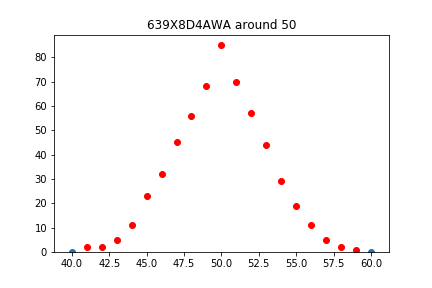
\includegraphics[width=\textwidth]{./images/639X8D4AWA_around_50.png}
		\end{subfigure}
		\begin{subfigure}{.47\textwidth}
			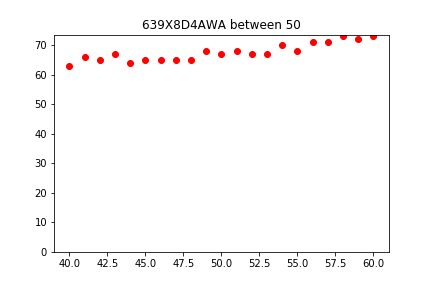
\includegraphics[width=\textwidth]{./images/639X8D4AWA_between_50.png}
		\end{subfigure}
		\caption{Participant with biggest score difference (s(around)-s(between))}
	\end{subfigure}
	\begin{subfigure}{\textwidth}
		\begin{subfigure}{.47\textwidth}
			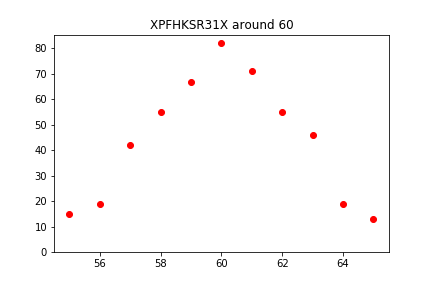
\includegraphics[width=\textwidth]{./images/XPFHKSR31X_around_60.png}
		\end{subfigure}
		\begin{subfigure}{.47\textwidth}
			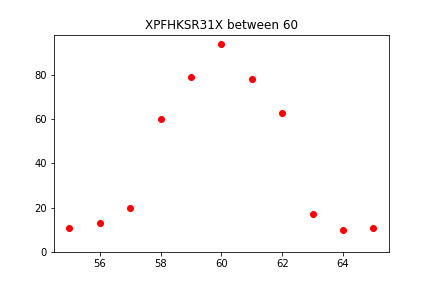
\includegraphics[width=\textwidth]{./images/XPFHKSR31X_between_60.png}
		\end{subfigure}
		\caption{Participant with smallest score difference (s(around)-s(between))}
	\end{subfigure}
\end{figure}
\end{minipage}\quad
\begin{minipage}{.35\textwidth}
	\begin{block}{Observation}
		\begin{itemize}
			\item the biggest bias toward a peaked \textit{around} appears bigger than the biggest bias toward a peaked \textit{between}...
			\item if not all the participants comply to our model, at least they do not exactly follow the inverse tendency!
		\end{itemize}
	\end{block}
\end{minipage}
\end{frame}

\begin{frame}{Study of \textit{between}-intervals (1)}
	\begin{block}{Goals}
		\begin{itemize}
			\item evaluate the performance of the participants for the \textit{between}-trials (interval task);
			\item study the different kinds of ``errors'' related to the \textit{between}-intervals;
			\item see whether there is a rationale behind these ``errors''.
		\end{itemize}
	\end{block}
	\begin{minipage}{.55\textwidth}
		\begin{figure}
		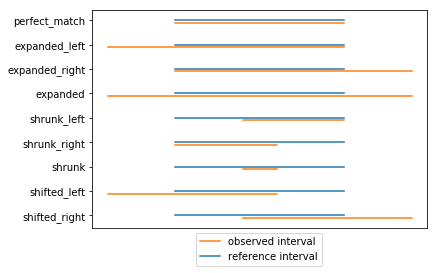
\includegraphics[width=\textwidth]{./images/memo_interval.png}
	\end{figure}
	\end{minipage}
\begin{minipage}{.4\textwidth}
	\begin{table}
		\centering
		\setlength\tabcolsep{3 pt}
		\small
	\begin{tabular}{c|cc}
		& Target & All \\ \hline
		\# of trials & 196 & 588 \\
		 \begin{tabular}{c}
			\# of non-\\overlapping
		\end{tabular} & 1 & 7 \\
	 \begin{tabular}{c}
		\% of non-\\overlapping
	\end{tabular} & 0.51 \% & 1.19 \%		
	\end{tabular}
\end{table}
\end{minipage}
\end{frame}
\begin{frame}{Study of \textit{between}-intervals (2)}
\begin{figure}
	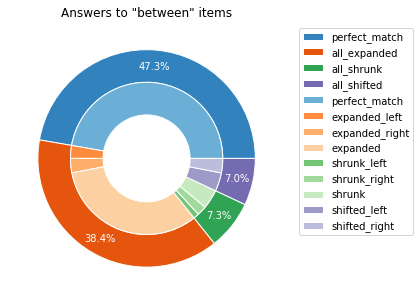
\includegraphics[width=.45\textwidth]{./images/between_items_int.png}
	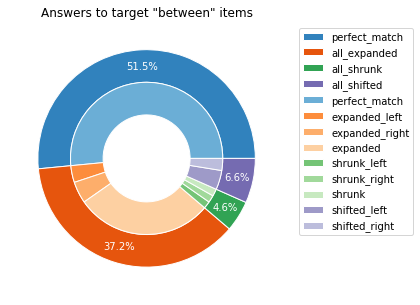
\includegraphics[width=.45\textwidth]{./images/target_between_items_int.png}
\end{figure}
\vspace{-5mm}
\begin{block}{Observations}
	\begin{itemize}
		\item perfect match in half of the cases;
		\item the predominant type of ``error'' is interval expansion, and especially cases of strict expansion (both sides);
		\item ``phantom readings'' (``at least(between(n, m))'', \cite{Marty2014}) are not prominent in our case...normal given syntactic structure!
	\end{itemize}
\end{block}
\end{frame}

\begin{frame}{Study of \textit{around}-intervals (1)}
\begin{block}{Goals}
	\begin{itemize}
		\item evaluate the performance of the participants for the \textit{around}-trials (interval task);
		\item study the different kinds of ``errors'' related to the \textit{around}-intervals;
		\item see whether there is a rationale behind these ``errors''.
	\end{itemize}
\end{block}
\begin{minipage}{.55\textwidth}
	\begin{figure}
		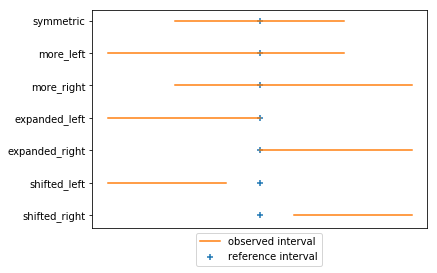
\includegraphics[width=\textwidth]{./images/memo_interval_around.png}
	\end{figure}
\end{minipage}
\begin{minipage}{.4\textwidth}
	\begin{table}
		\centering
		\setlength\tabcolsep{3 pt}
		\small
		\begin{tabular}{c|cc}
			& Target & All \\ \hline
			\# of trials & 196 & 588 \\
			\begin{tabular}{c}
				\# of non-\\overlapping
			\end{tabular} & 9 & 29 \\
			\begin{tabular}{c}
				\% of non-\\overlapping
			\end{tabular} & 4.59 \% & 4.93 \%		
		\end{tabular}
	\end{table}
\end{minipage}
\end{frame}

\begin{frame}{Study of \textit{around}-intervals (2)}
\begin{figure}
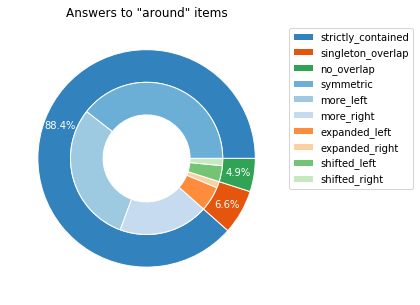
\includegraphics[width=.45\textwidth]{./images/around_items_int.png}
\includegraphics[width=.45\textwidth]{./images/target_around_items_int.png}
\end{figure}
\vspace{-5mm}
\begin{block}{Observations}
\begin{itemize}
	\item $n$ ``strictly'' contained in the interval (not a bound) in almost 90\% of the cases;
	\item bias toward left: cannot be explained by log scale...
	\item  granularity? Not only because targets are skewed;u
	\item no ``phantom readings''.
\end{itemize}
\end{block}
\end{frame}

\begin{frame}{Exploratory analysis -- Effect of available alternatives}
\begin{block}{Available alternatives and order effects}
	\begin{itemize}
		\item some participants may face the first target item (\textit{around}) having seen all kinds of approximators (\textit{around}, \textit{between} and \textit{almost}), or a strict subset of them;
		\item given what they know about the possible alternatives, they would want to give contrastive distributions;
	\end{itemize}
\end{block}
\begin{minipage}{.45\textwidth}
	\begin{figure}
		\centering
	\includegraphics[width=\textwidth]{./images/sensitivity_competitors.png}
\end{figure}
\end{minipage}\quad
\begin{minipage}{.5\textwidth}
	\begin{block}{Test}
		\begin{itemize}
			\item we compared the peakedness of target \textit{around} items depending on the alternatives already presented (MW+Bonferroni)
			\item no huge difference.
		\end{itemize}
	\end{block}
\end{minipage}
\end{frame}
\end{document}
